\documentclass[a4paper,12pt]{article}

\usepackage[spanish]{babel}
\usepackage[utf8]{inputenc}
\usepackage{amsmath, amssymb}
\usepackage{geometry}
\usepackage{graphicx}
\usepackage{amssymb}
\usepackage{stmaryrd}
\usepackage{tcolorbox}
\geometry{margin=2.5cm}

\title{Resumen: Sintaxis Abstracta y Semántica}
\author{}
\date{}

\begin{document}

\maketitle

\section{Gramáticas Abstractas}

Las gramáticas permiten definir los lenguajes formales. Se distingue entre:

\begin{itemize}
    \item \textbf{Sintaxis concreta:} define cómo se escriben las expresiones (paréntesis, precedencia).
    \item \textbf{Sintaxis abstracta:} describe la estructura esencial de las expresiones.
\end{itemize}

Ejemplo de gramática abstracta:

\begin{align*}
\langle intexp \rangle ::= &\ 0 \mid 1 \mid 2 \mid \dots \\
&\mid -\langle intexp \rangle \\
&\mid \langle intexp \rangle + \langle intexp \rangle \\
&\mid \langle intexp \rangle * \langle intexp \rangle
\end{align*}

Las gramáticas abstractas pueden ser ambiguas, lo cual se refleja en distintos árboles sintácticos para una misma expresión.

\section{Función Semántica}

La semántica denotacional se define mediante una función:

\[
[[\cdot]] : \langle intexp \rangle \rightarrow \mathbb{Z}
\]

Ejemplo de ecuaciones semánticas:

\begin{align*}
[[0]] &= 0 \\
[[ -e ]] &= -[[e]] \\
[[ e + e']] &= [[e]] + [[e']] \\
[[ e * e']] &= [[e]] * [[e']]
\end{align*}

\subsection{Conceptos importantes}

\begin{itemize}
    \item \textbf{Metacircularidad:} mismos símbolos en lenguaje y metalenguaje.
    \item \textbf{Metavariables:} variables del metalenguaje (ej: $e, e'$).
    \item \textbf{[[e]]:} Es un abuso de notación que se resuelve escribiendo $[[\lfloor e \rfloor ]]$.
\end{itemize}

\section{Dirección por Sintaxis y Composicionalidad}

Una definición es \textbf{dirigida por sintaxis} si:

\begin{itemize}
    \item Hay una ecuación por cada producción.
    \item El significado depende solo de las subexpresiones.
\end{itemize}

Esto garantiza:

\begin{itemize}
    \item Existencia y unicidad del significado.
    \item \textbf{Composicionalidad:} el significado de una expresión depende solo del de sus partes.
\end{itemize}

\section{Variables y Estados}

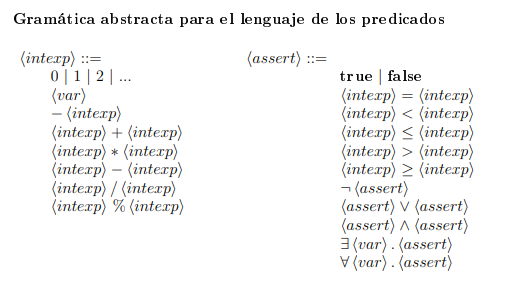
\includegraphics[width=1\textwidth]{./gramaticaparaPredicados.png}

Se introduce el concepto de estado:

\[
\Sigma = \langle var \rangle \rightarrow \mathbb{Z}
\]

El significado de una expresión depende del estado:

\[
[[e]] : \Sigma \rightarrow \mathbb{Z}
\]

Actualización de estados: definimos la siguiente operación sobre estados. Sea $\sigma \in \Sigma$ un estado, $v$ una variable y $n$ un entero. Entonces $[\sigma | v : n]$ es un estado que coincide con $\sigma$ en todas las variables salvo posiblemente en $v$, donde este nuevo estado tiene asignado $n$. En símbolos:

\[
[\sigma | v : n]w \quad = \quad \text{si } (w = v) \text{ entonces } n \text{ sino } \sigma w
\] (pregunta por $w$)

\begin{tcolorbox}[title=Notaciones de autora]
\noindent La fun semántica $\llbracket x+5 \rrbracket_\sigma$ si se tiene $x + 5$ por sí sola no vale nada.

\begin{itemize}
    \item[$\hookrightarrow$] \textbf{Estado $\sigma$:} memoria, valor de cada variable.
    \item[$\hookrightarrow$] \textbf{función:} dado un estado $\sigma$ devuelve un número entero.
    \item[$\hookrightarrow$] $\llbracket \cdot \rrbracket$: separa el mundo del código (sintaxis) del mundo de los números (semántica).
\end{itemize}

\medskip

\noindent $\llbracket e \rrbracket \sigma$: El valor de la expresión $e$ evaluada bajo el estado $\sigma$.

\noindent $[\sigma | v : n] \to$ nuevo estado, casi idéntico a $\sigma$ pero $v$ ahora vale $n$.
\end{tcolorbox}
\section{Expresiones Booleanas}

Se define:

\[
[[\cdot]] : \langle assert \rangle \rightarrow \Sigma \rightarrow \{V, F\}
\]

Ejemplos:

\begin{align*}
[[true]]_\sigma &= V \\
[[e = e']]_\sigma &= ([[e]]_\sigma = [[e']]_\sigma) \\
[[p \land q]]_\sigma &= ([[p]]_\sigma \land [[q]]_\sigma) \\
[[\forall v.p]]_\sigma &= \forall n \in \mathbb{Z}. [[p]]_{\sigma[v:n]}
\end{align*}

\section{Variables Libres y Ligadas}

\begin{itemize}
    \item \textbf{Ocurrencia ligadora:} una ocurrencia ligadora de una variable es la que se encuentra inmediatamente después de un cuantificador ($\forall$ o $\exists$).
    
    \item \textbf{Alcance de una ocurrencia ligadora:} En $\forall v. p$ o $\exists v. p$, el predicado $p$ es el alcance de la ocurrencia ligadora de $v$.
    
    \item \textbf{Ocurrencia ligada:} cualquier ocurrencia de $v$ en el alcance de una ocurrencia ligadora de $v$ es una ocurrencia ligada de $v$. Dicha ocurrencia ligada puede estar en más de un alcance de ocurrencias ligadoras de $v$. Se dice que está ligada por la ocurrencia ligadora de menor alcance.
    
    \item \textbf{Ocurrencia libre:} una ocurrencia de una variable que no es ligadora ni ligada es una ocurrencia libre.
    
    \item \textbf{Variable libre:} una variable que tiene ocurrencias libres es una variable libre.
    
    \item \textbf{Una expresión cerrada} es una que no tiene variables libres.
\end{itemize}

Se define el conjunto de variables libres $FV$ por recursión sobre la sintaxis.
\begin{align*}
    FV \lfloor n \rfloor &= \emptyset \\
    FV \ v &= \{v\} \\
    FV (-e) &= FV \ e \\
    FV (e + e') &= FV \ e \cup FV \ e' \\
    &\vdots
\end{align*}

y para expresiones booleanas:

\begin{align*}
    FV \ \textbf{true} &= \emptyset \\
    FV \ \textbf{false} &= \emptyset \\
    FV (e = e') &= FV \ e \cup FV \ e' \\
    &\vdots \\
    FV (\neg p) &= FV \ p \\
    FV (p \wedge q) &= FV \ p \cup FV \ q \\
    &\vdots \\
    FV (\forall v. \ p) &= (FV \ p) - \{v\} \\
    FV (\exists v. \ p) &= (FV \ p) - \{v\}
\end{align*}

\section{Sustitución}

 Comenzamos definiendo sustitución como una función de variables en expresiones:

\[
\Delta : \langle var \rangle \rightarrow \langle intexp \rangle
\]

Definimos ahora el operador sustitución, que opera sobre expresiones enteras (términos) y expresiones booleanas (predicados):

Para expresiones enteras, $\_ / \_ \in \langle intexp \rangle \times \Delta \to \langle intexp \rangle$ se define mediante las siguientes igualdades:

\begin{align*}
    0/\delta &= 0 \\
    1/\delta &= 1 \\
    &\vdots \\
    v/\delta &= \delta v \\
    (-e)/\delta &= -(e/\delta) \\
    (e + f)/\delta &= (e/\delta) + (f/\delta) \dots
\end{align*}

Intuitivamente podemos pensar que una sustitución se propaga por toda la estructura de la expresión entera salvo cuando se encuentra con una variable, en cuyo caso reemplaza según indica la sustitución.

\subsection{Problema de captura}

Ocurre cuando una variable libre pasa a estar ligada tras una sustitución.

Una solución es renombrar la variable ligada y luego sustituir. Otra posibilidad es hacer las dos cosas simultáneamente. Si bien es más complicado, es lógico hacerlo así ya que estamos definiendo justamente la sustitución. Definimos entonces, para $Q = \forall, \exists$:

\[
(Qv. b) / \delta = Qv_{new} . (b / [\delta | v : v_{new}])
\]

donde $v_{new}$ es una variable \textit{nueva} y $[\delta | v : v_{new}]$ ya se definió: sustituye parecido a $\delta$, salvo que a la variable $v$ la reemplaza por $v_{new}$. Si no elegimos cuidadosamente a $v_{new}$, el problema de la captura persiste. 

Para finalizar, entonces, tenemos las ecuaciones
\begin{align*}
    (\forall v . \ b) / \delta &= \forall v_{new} . \ (b / [\delta | v : v_{new}]) \text{ donde } v_{new} \notin \bigcup_{w \in FV(b) - \{v\}} FV(\delta w) \tag{Nota 1}\\
    (\exists v . \ b) / \delta &= \exists v_{new} . \ (b / [\delta | v : v_{new}]) \text{ donde } v_{new} \notin \bigcup_{w \in FV(b) - \{v\}} FV(\delta w)
\end{align*}

\begin{tcolorbox}[title=Notaciones de autora]
    Nota 1: Intuitivamente $(b / [\delta | v : v_{new}])$ es: Hacé todos los reemplazos que decía $\delta$ pero si encontrás a $v$ dentro de $b$, cambiala por $v_{new}$. 
    Además $v_{new}$ no debe de estar en el conjunto de variables libres de las expresiones que sustituyen a las variables libres de $b$ distintas de $v$ es para evitar el problema de captura.
\end{tcolorbox}

\section{Propiedades Semánticas}

\begin{itemize}
\item \textit{Coincidencia}, expresa que el significado de una frase no puede depender de variables que no ocurran libres en la misma. 
\item \textit{Renombre}, asegura que el significado no depende de las variables ligadas de una frase.
\end{itemize}

\medskip

\noindent \textbf{Teorema de Coincidencia (TC).} Si dos estados $\sigma$ y $\sigma'$ coinciden en las variables libres de $p$, entonces da lo mismo evaluar $p$ en $\sigma$ o $\sigma'$. En símbolos:
\[
(\forall w \in FV(p) \ldotp \sigma w = \sigma' w) \implies \llbracket p \rrbracket \sigma = \llbracket p \rrbracket \sigma'
\]

En particular, TC implica que el valor de un término cerrado es el mismo en cualquier estado, es decir, no depende del estado.

\medskip

\noindent \textbf{Teorema de Renombre (TR).} Los nombres de las variables ligadas no tienen importancia. En símbolos,
\[
u \notin FV(q) - \{v\} \implies \llbracket \forall u \ldotp q / v \to u \rrbracket = \llbracket \forall v \ldotp q \rrbracket
\]

\medskip

Para la prueba de las mismas, debemos recurrir a propiedades más generales.

\medskip

\noindent \textit{Teorema de Sustitución (TS).} Si aplico la sustitución $\delta$ a $p$ y luego evalúo en el estado $\sigma$, puedo obtener el mismo resultado a partir de $p$ sin sustituir si evalúo en un estado que hace el trabajo de $\delta$ y de $\sigma$ (en las variables libres de $p$). En símbolos:
\[
(\forall w \in FV(p) \ldotp \llbracket \delta w \rrbracket \sigma = \sigma' w) \implies \llbracket p / \delta \rrbracket \sigma = \llbracket p \rrbracket \sigma'
\tag{Nota 2} \] 

\noindent \textit{Abreviatura.} Si consideramos $id$ como la sustitución identidad, que mapea cada variable $v$ en la expresión $v$, entonces escribiremos $v_0 \to e_0, \dots, v_{n-1} \to e_{n-1}$ para abreviar $[id | v_0 : e_0 | \dots | v_{n-1} : e_{n-1}]$.

\medskip

\noindent \textit{Teorema de Sustitución Finita (TSF, corolario de TS).}
\[
\llbracket p / v_0 \to e_0, \dots, v_{n-1} \to e_{n-1} \rrbracket \sigma = \llbracket p \rrbracket [\sigma | v_0 : \llbracket e_0 \rrbracket \sigma | \dots | v_{n-1} : \llbracket e_{n-1} \rrbracket \sigma]
\]

\begin{tcolorbox}[title=Notaciones de autora]
\begin{itemize}
    \item Nota 2: $\forall$ variable $w$ que sea libre en $p$, si el valor de la expresión que sustituye a $w$ ($\delta w$) evaluada en el estado $\sigma$ es igual al valor que el estado $\sigma'$ le asigna a $w$, $\longrightarrow$ el significado de $p$ tras aplicarle la sustitución $\delta$ y evaluarla en el estado $\sigma$ es lo mismo que evaluar $p$ en el estado $\sigma'$.
    \item \noindent \textbf{Ej:} $p = x + 10$, \quad $x \to y * 2$, \quad $\sigma(y) = 3$

\medskip

\noindent \textbf{camino 1:} 
$\llbracket p/\delta \rrbracket \sigma \to (x+10) \to ((y*2)+10) \to \llbracket (3*2) + 10 \rrbracket = 16$

\medskip

\noindent \textbf{camino 2:} Crear $\sigma'$ donde $x$ tenga el valor procesado:
\begin{align*}
    \therefore \sigma'(x) &= \llbracket (y*2) \rrbracket \sigma \\
    \therefore \sigma'(x) &= 6
\end{align*}

\noindent $\therefore \llbracket x + 10 \rrbracket \sigma' = \llbracket 6 + 10 \rrbracket = 16$
\end{itemize}
\end{tcolorbox}


\end{document}